

\section{Experiments}
\label{sec:expr}
We have prototyped our language, execution model, and some of our
optimizations as modifications to the \Pitu system. Our
prototype takes as input \Dlog programs, performs rule localization, and generates a dataflow graph
consisting of \Pitu \xspace{\em elements}. Each element is a node in the dataflow
graph, and performs tasks such as queuing, network processing and
traditional relational operations like joins and aggregations.

The generated execution plan is structurally similar to
Figure~\ref{Dataflow1}, where there are rule strands comprising
chains of elements. Each rule strand takes as input a queue,
corresponding to new tuples for each strand. Our current
implementation uses the PSN algorithm at the tuple granularity. A
new tuple is dequeued and processed by the rule strand to generate new
tuples which are then enqueued at the same node or sent as a network
message for further processing at another node.

Beyond validating our language and implementation, the main goal of our evaluation
is to verify the effectiveness of several of the proposed
optimizations. In evaluating our system, the main metrics that we use
are: 

\vspace{1pt}
\noindent {\bf Convergence time: }The time taken for the query execution
to generate all the query results.

\vspace{1pt}
\noindent {\bf Communication overhead: }The number of bytes transferred
  for each query. We consider both aggregate communication overhead (MB), as well as
  per-node bandwidth (kBps).


In summary, we find:
  
\begin{CompactEnumerate}
\item The aggregate selections optimization reduces communication overhead. Using {\em
  periodic aggregate selections} reduces this overhead further. 

\item The use of magic sets and predicate reordering reduces communication overhead when only a limited number of paths
  are queried. 

\item Multi-query sharing techniques such as query result caching and
  opportunistic result caching demonstrate the potential to reduce communication
  overhead when there are several concurrent queries.

\item On a network with bursty updates, incremental query evaluation
  techniques can recompute paths at a fraction of the cost of
  recomputing the queries from scratch.
  
\end{CompactEnumerate}

%In practice,
%  we have scaled \Sys on up to a thousand processes running on a single
%  machine without any network emulation.} 

\subsection{Setup}

Our experiments are conducted by running our modified \Pitu on 100 nodes
on the Emulab~\cite{emulab}
testbed. This testbed emulates realistic latency and bandwidth constraints seen on the Internet,
  yet provides repeatable experiments under a controlled environment. As input to the Emulab testbed, we use transit-stub
topologies generated using GT-ITM~\cite{gtitm}, a package that is widely used to model
Internet topologies. Our topology has four transit nodes, eight nodes
per stub and three stubs per transit node. Latency between transit nodes
  is $50$ ms, latency between transit nodes and their stub nodes is $10$
ms, and latency between any two nodes in the same stub is $2$
ms. The link capacity is set to $10$ Mbps.

We construct an overlay network over the base GT-ITM topology where
each node is assigned to one of the stub nodes. Each overlay node runs
\Sys on one Emulab machine, and picks four randomly selected
neighbors. Each node has four link tuples, one for each neighbor. Each
link tuple has metrics that include latency (based on the underlying GT-ITM
topology), reliability (link loss correlated with latency),
and a randomly generated value.  

We base our workload primarily on routing
protocols~\cite{declareRoute}, and benchmark four variants of the
same {\em shortest-path} query, differing in the link metric each
seeks to minimize. On all our graphs, we label these queries by their
link metric: {\em Hop-Count}, {\em Latency}, {\em Reliability} and
{\em Random}, respectively. Note that {\em Random} serves as our
stress case: we expect it to have the worst performance among all
queries, because aggregate selections are less
likely to be effective when the aggregate metric is uncorrelated with
the network latency, which determines tuple arrival order during query
execution.
%. These queries are used to compute the optimal paths between all pairs
%  of nodes based on various link metrics. 




%  to less effective aggregate selections. When completed, each of these
%  queries would compute the optimal paths for the {\em fewest
%    hop-count}, {\em lowest aggregate latency}, {\em most
%  reliable} and {\em lowest aggregate random}.  


\subsection{Aggregate Selections}
\label{subsec:expr:aggsel}


\begin{figure}[ht]
\centering
 \begin{minipage}{.45\linewidth}
  \begin{center}
    \epsfig{file=graphs/baseline/bw.ps,width=1.18in,angle=-90}
    \small{\caption{\label{baseline-bw}\emph{\small Per-node Bandwidth (kBps).}}}
    \end{center}
 \end{minipage}
\hfill
 \begin{minipage}{.45\linewidth}
  \begin{center}
    \epsfig{file=graphs/baseline/results.ps,width=1.18in,angle=-90}
    \small{\caption{\label{baseline-convergence}\emph{\small
    Query results over time (seconds).}}}
  \end{center}
 \end{minipage}
\end{figure}

We first investigate the effectiveness of aggregate selections for
different queries. Figure~\ref{baseline-bw} shows the per-node
bandwidth usage against time for the four
queries. Figure~\ref{baseline-convergence} shows the percentage of
eventual best paths completed against time. Our results show that {\em
Hop-Count} converges the most quickly in $4.4$ seconds, followed by
{\em Latency} and {\em Reliability} in $4.9$ seconds and $4.8$ seconds
respectively. {\em Random} has the worst convergence time
of $5.8$ seconds.

During query execution, the communication overhead incurred by all
four queries shows a similar trend
(Figure~\ref{baseline-bw}). Initially, the communication overhead
increases as more and more paths (of increasing length) are derived. After
it peaks at around $19 kBps$ per-node, the communication overhead
decreases, as fewer and fewer optimal paths are left to be derived. In
terms of aggregate communication overhead, {\em Random} incurs the
most overhead ($4.1$ MB), while {\em Hop-Count}, {\em Latency} and
{\em Reliability} use $2.6$ MB, $3.1$ MB and $3.2$ MB,
respectively. The relatively poor performance of {\em Random} is due
to the lack of correlation between the metric and network latency,
leading to a greater tendency for out-of-order arrival of path tuples
that results in less effective use of aggregate selections.


%\subsubsection{Periodic Aggregate Selections}

\begin{figure}[ht]
\centering
 \begin{minipage}{.45\linewidth}
  \begin{center}
    \epsfig{file=graphs/dynamic/bw-3.ps,width=1.18in,angle=-90}
    \small{\caption{\label{periodic-bw}\emph{\small Per-node Bandwidth (kBps).}}}
    \end{center}
 \end{minipage}
\hfill
 \begin{minipage}{.45\linewidth}
  \begin{center}
    \epsfig{file=graphs/dynamic/results-3.ps,width=1.18in,angle=-90}
    \small{\caption{\label{periodic-convergence}\emph{\small
    Query results over Time (seconds).}}}
  \end{center}
 \end{minipage}
\end{figure}

The results in Figures~\ref{periodic-bw} and
\ref{periodic-convergence} illustrate the effectiveness of 
the {\em periodic aggregate selections} approach, as described in
Section~\ref{subsec:aggregateSelections}.  In particular, this
approach reduces the bandwidth usage of {\em Hop-Count}, {\em
Latency}, {\em Reliability} and {\em Random} by $17$\%, $12$\%, $16$\%
and $29$\%, respectively. {\em Random} not only shows the greatest
reduction in communication overhead, its convergence time also reduces from $5.8$
seconds to $5$ seconds. 
%In all experiments we use a wait period of 300
%ms.

%This demonstrate the effectiveness of performing aggregate
%  selections in batches, by buffering up tuples before computing the
%  optimal paths to be sent to neighboring nodes.

\subsection{Magic Sets and Predicate Reordering}
\label{subsec:expr:caching}

\begin{figure}[ht]
\centering
 \begin{minipage}{.45\linewidth}
  \begin{center}
    \epsfig{file=graphs/magiccache/queryBW_random100.ps,width=1.18in,angle=-90}
    \small{\caption{\label{ms-bw}\emph{\small Aggregate communication overhead (MB) with and
    without magic sets and caching}.}}
    \end{center}
 \end{minipage}
\hfill
 \begin{minipage}{.45\linewidth}
  \begin{center}
    \epsfig{file=graphs/correlate/bw-corrshare3.ps,width=1.18in,angle=-90}
    \small{\caption{\label{opportunistic-bw300}\emph{\small
    Per-node Bandwidth (kBps) for message sharing (300 ms delay).}}}
  \end{center}
 \end{minipage}
%\hfill
% \begin{minipage}{.3\linewidth}
%  \begin{center}
%    \epsfig{file=graphs/correlate/bw-corrshare0.05.ps,width=1.5in,angle=-90}
%    \small{\caption{\label{opportunistic-bw50}\emph{\small Per-node Bandwidth (kBps) for
%    correlated sharing (50 ms delay)}}}
%    \end{center}
% \end{minipage}
\end{figure}

Next, we study the effectiveness of combining the use of magic sets
and predicate reordering for lowering communication overhead when the
queries are constrained by randomly chosen sources and
destinations. Our workload consists of queries that request
source-to-destination paths based on the {\em Hop-Count} metric. For
each query, we execute the {\em magic-shortest-path} query
(Section~\ref{sec:magic}). 

Figure~\ref{ms-bw} shows the aggregate communication overhead as the number of
queries increases.  The {\em No-MS} line represents our baseline, and
shows the communication overhead in the absence of rewrites (this
essentially reduces to computing all-pairs least-hop-count). The {\em
MS} line shows the communication overhead when running the optimized
query with no sharing across queries. When there are few queries, the
communication overhead of {\em MS} is significantly lower than that of
{\em NO-MS}. As the number of queries increases, the communication
overhead of {\em MS} increases linearly, exceeding {\em No-MS} after
$170$ queries.

%\subsubsection{Magic Sets with Caching}
%\label{subsec:expr:magic}

In addition, Figure~\ref{ms-bw} also illustrates the effectiveness of
caching (Section~\ref{subsec:multiQuerySharing}). The {\em MSC} line
shows the aggregate communication overhead for magic sets with caching. For
fewer than $170$ queries, there is some overhead associated with
caching. This is due to false positive cache hits, where a cache
result does not contribute to computing shortest paths. However, as
the number of queries increases, the overall cache hit rate improves,
resulting in a dramatic reduction of bandwidth. 
When limiting the choice of destination nodes to $30$\% ({\em
MSC-30\%}) and $10$\% ({\em MSC-10\%}), the communication overhead
levels of at $1.8$ MB, and $1$ MB, respectively. The smaller the set
of requested destinations, the higher the cache hit rate, and
the greater the opportunity for sharing across different queries.
These results are consistent with the results obtained by Loo
\textit{et~al.}~\cite{declareRoute} in a similar experiment,
using the PIER~\cite{pierCidr} simulator.


\subsection{Opportunistic Message Sharing}
\label{subsec:expr:correlated}

We study the impact of performing opportunistic message sharing across
concurrent queries that have some correlation in the messages being
sent. Figure~\ref{opportunistic-bw300} shows per-node bandwidth
usage for running the queries on different metrics
concurrently. To facilitate sharing, we delay each outbound tuple by
$300$ms in anticipation of possible sharing opportunities. The {\em
Latency}, {\em Reliability} and {\em Random} lines show the bandwidth
usage of each query individually. The {\em No-Share} line shows
the total aggregate bandwidth of these three queries without
sharing. The {\em Share} line shows the aggregate bandwidth
usage with sharing. Our results clearly demonstrate the
potential effectiveness of message sharing, which reduces the peak of
the per-node communication overhead from 27 kBps to 16 kBps, and the
total communication overhead by 34\%.

%We repeat the experiment with a lower outbound delay of $50$ ms, and
% observed that there is less sharing achievable across queries. The peak
% per-node bandwidth usage attained with sharing is 22 kBps, which
% is only marginally lower compared to no sharing. The aggregate
% bandwidth usage is reduced by 18\%, which is far less than when the delay is $300$ ms. This clearly
% demonstrates the usefulness in delaying outbound tuples in
% order to facilitate sharing. Determining the correct period at
% runtime based on the query workload is an interesting area for further exploration.

\subsection{Incremental Query Evaluation}
\label{subsec:expr:dynamic}

\begin{figure}[ht]
\centering
 \begin{minipage}{.45\linewidth}
  \begin{center}
    \epsfig{file=graphs/dynamic/bw-random-burb-10.ps,width=1.18in,angle=-90}
    \small{\caption{\label{bursty-bw1}\emph{\small Per-node Bandwidth (kBps) for
    periodic link updates on latency metric (10s update interval).}}}
    \end{center}
 \end{minipage}
\hfill
 \begin{minipage}{.45\linewidth}
  \begin{center}
    \epsfig{file=graphs/dynamic/bw-latency-burb-random-vary.ps,width=1.18in,angle=-90}
    \small{\caption{\label{bursty-bw2}\emph{\small
    Per-node Bandwidth (kBps) for periodic link updates (interleaving 2s and 8s
    update interval).}}}
  \end{center}
 \end{minipage}
\end{figure}


In our final experiment, we examine the overhead of incrementally
maintaining query results in a dynamic network. We run the queries
over a period of time, and subject the network to burst updates as
described in Section~\ref{sec:dynamic}.  Each update burst involves
randomly selecting 10\% of all links, and then updating the cost
metric by up to 10\%. We use the shortest-path random metric since it
is the most demanding in terms of bandwidth usage and
convergence time.

Figure~\ref{bursty-bw1} plots the per-node communication overhead,
when applying a batch of updates every $10$ seconds. Two points are worth
noting. First, the time it takes the query to converge after a burst
of updates is well within the $5$ second convergence time of running the
query from scratch (Figure~\ref{periodic-convergence}). This is
reflected in the communication overhead, which increases sharply after
a burst of updates is applied, but then disappears long before the next
burst of updates (Figure~\ref{bursty-bw1}). Second, each burst peaks
at $6 kBps$, which is only 32\% of the peak bandwidth and 26\% of the
aggregate bandwidth of the original computation. Our results clearly
demonstrate the usefulness of performing incremental query evaluation
in response to changes in the network, as opposed to recomputing the
queries from scratch.     

We repeat our experiment on a more demanding update workload
(Figure~\ref{bursty-bw2}), where we interleave update intervals that
are $2$ seconds and $8$ seconds, the former interval being less than
the from-scratch convergence time of $5$ seconds. We observe that
despite the fact that bursts are sometimes occurring faster than
queries can run, bandwidth usage is similar to the less
demanding update workload. When the update interval is $2$ seconds, we
notice periods of sustained bandwidth usage, however the peak
usage remains at $6$ kBps as before.
%When the interval is subsequently increased to $8$ seconds, the query computation
%quiesces as shown by the reduction of bandwidth usage to $0$ kBps. 




 
%At the same
% time, there is also no noticeable improvement to the convergence
% time relative to the previous experimental setup, as the extra messages
% negate any impact of lowering the periodic interval. Figuring out the
% correct interval at runtime base on parameters such as opportunities for sharing, allowing for
% out-of-sync queries issued at different times to ``catch-up and
% share'', and adapting based on the rate of change in the
% network are interesting aspects of adaptive query processing for further exploration.


%\subsubsection{Hybrid Rewrites}
%\label{subsec:expr:hybrid}

%TO FILL IN. 

%Compare bandwidth and convergence with all-pairs shortest path
%computation (Figure~\ref{zone-bw}).

%Compare with flood-based source routing and show that this is cheaper in
%bandwidth (Figure~\ref{zone-route}). 


%\subsection{Summary}
%Summarize the key points in evaluation.



%\subsubsection{Gossip-based Approximations}
%\label{subsec:expr:hybrid}

%OPTIONAL if time permits.

%Graph for gossip:

%\begin{itemize}
%\item Y-axis: Bandwidth / Path length
%\item X-axis: Time
%\end{itemize}

%Repeat for different gossip rate (\% of paths not propagated to neighbors). Show
%tradeoffs of path quality and bandwidth. 





%\subsection{Query Approximations}
%\label{subsec:expr:queryApprox}

%\begin{itemize}
%\item Y-axis: Convergence / Bandwidth 
%\item X-axis: Time 
%\end{itemize}

%Demonstrate bandwidth reduction vs loss of results quality. Show CDF of
%computed path costs for approximation and without approximation.


%\subsection{Multi-Objective Queries}
%\label{subsec:expr:multiObj}

%Optional. Show highly correlated (latency, loss-rate) multi-objective
%can result in savings. 


% LocalWords:  dataflow PSN kBps bursty Emulab ITM Mbps bw MSC Loo al
